% Classification of Fermi-LAT 4FGL-DR4 sources: final results.
% Build from this folder:  latexmk -pdf fermi_classification.tex
% Figures: figures/*.png are copied from the run's plots; figures/*.pdf come from make_figures.py.
\documentclass[aspectratio=169, 10pt]{beamer}

\usetheme{CambridgeUS}
\usecolortheme{beaver}
\setbeamertemplate{navigation symbols}{}
\setbeamertemplate{footline}[frame number]

\usepackage[utf8]{inputenc}
\usepackage[T1]{fontenc}
\usepackage{graphicx}
\usepackage{booktabs}
\usepackage{amsmath, amssymb}
\usepackage{tikz}
\usetikzlibrary{positioning, arrows.meta}
\graphicspath{{figures/}}
\hypersetup{pdftitle={Classification of Fermi-LAT 4FGL-DR4 sources}, pdfauthor={Filippo Graci}}

\newcommand{\cls}[1]{\texttt{#1}}
\tikzset{
  box/.style={draw=darkred!70, rounded corners=2pt, fill=darkred!6, align=center,
              font=\scriptsize, inner sep=3pt, minimum height=0.6cm},
  arr/.style={-{Stealth[length=4pt]}, darkred!70},
}

\title[Fermi 4FGL classification]{Classification of Fermi-LAT 4FGL-DR4 sources}
\subtitle{Flat and hierarchical models, validated on held-out data}
\author[F. Graci]{Filippo Graci}
\institute[UniPV]{Università di Pavia}
\date{November 2026}

\begin{document}

\begin{frame}
  \titlepage
\end{frame}

\begin{frame}{Outline}
  \tableofcontents
\end{frame}

% =====================================================================
\section{Problem and data}

\begin{frame}{The question}
  \begin{itemize}
    \item The Fermi-LAT 4FGL-DR4 catalog (\cls{gll\_psc\_v35.fit}) lists 7,194 gamma-ray sources.
    \item 4,631 are associated with a known counterpart and have a class (\cls{CLASS1}).
          2,563 are unassociated.
    \item Goal 1: learn the class from the gamma-ray properties alone (spectrum, variability,
          localization, position), using the associated sources.
    \item Goal 2: predict a class for the unassociated sources, with an honest estimate of how
          reliable those predictions are.
    \item Question: does a hierarchical classifier, which first separates broad families of
          sources, beat a single flat classifier?
  \end{itemize}
  \vspace{0.3cm}
  \small Every number in this talk comes from one final run, documented in \cls{RESULTS.md}.
\end{frame}

\begin{frame}{Classes used (Setup B)}
  \begin{columns}[T]
    \begin{column}{0.55\textwidth}
      \scriptsize
      \begin{tabular}{llr}
        \toprule
        Superclass & Classes & Sources \\
        \midrule
        Blazar, high energy peak & \cls{fsrq} (with \cls{ssrq}, \cls{css}) & 828 \\
        Blazar, low energy peak & \cls{bll} & 1,490 \\
        Other AGN & \cls{rdg}, \cls{nlsy1}, \cls{agn}, \cls{sey} & 73 \\
        Isolated pulsars & \cls{msp}, \cls{psr}, \cls{glc} & 361 \\
        Binary systems & \cls{hmb}, \cls{bin}, \cls{lmb}, \cls{nov} & 38 \\
        SNR and PWN & \cls{snr}, \cls{pwn} & 66 \\
        Galactic extended & \cls{sbg}, \cls{gal}, \cls{sfr} & 20 \\
        \midrule
        Total & 18 classes & 2,876 \\
        \bottomrule
      \end{tabular}
    \end{column}
    \begin{column}{0.42\textwidth}
      \small
      \begin{itemize}
        \item Excluded: \cls{bcu} (1,623 blazars of uncertain type) and \cls{spp} (132 sources
              of uncertain nature). Neither has a well-defined class to learn.
        \item \cls{ssrq} and \cls{css} are merged into \cls{fsrq}.
        \item The superclasses define the branches of the hierarchical models.
      \end{itemize}
    \end{column}
  \end{columns}
\end{frame}

\begin{frame}{Severe class imbalance}
  \begin{columns}[c]
    \begin{column}{0.62\textwidth}
      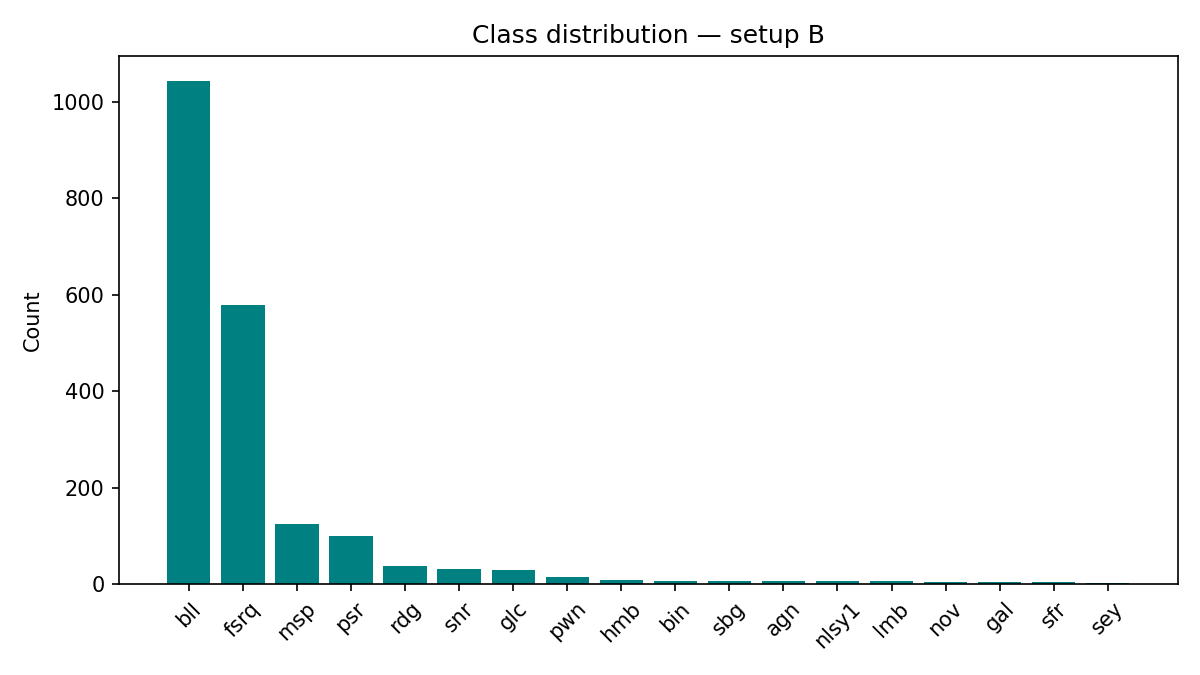
\includegraphics[width=\linewidth]{class_distribution_train.png}
    \end{column}
    \begin{column}{0.36\textwidth}
      \small
      \begin{itemize}
        \item Training split shown: two blazar classes make up 80\% of the sources.
        \item Ten of the 18 classes have three or fewer sources in the test set.
        \item Accuracy is dominated by \cls{bll} and \cls{fsrq}, so models are selected on
              macro-F1, which weights every class equally.
      \end{itemize}
    \end{column}
  \end{columns}
\end{frame}

\begin{frame}{Three model architectures}
  \centering
  \begin{tikzpicture}[node distance=0.45cm and 0.25cm]
    % flat
    \node[font=\small\bfseries] (t1) at (0, 0) {Flat (fine)};
    \node[box, below=0.3cm of t1, minimum width=2.6cm] (f1) {one classifier\\18 classes};
    % merged
    \node[font=\small\bfseries] (t2) at (4.6, 0) {2-level (merged)};
    \node[box, below=0.3cm of t2, minimum width=2.6cm] (r2) {router\\7 superclasses};
    \node[box, below=of r2, minimum width=3.2cm] (b2) {one model per superclass\\(blazars pass through)};
    \draw[arr] (r2) -- (b2);
    % 3 level
    \node[font=\small\bfseries] (t3) at (10.2, 0) {3-level};
    \node[box, below=0.3cm of t3, minimum width=2.6cm] (g3) {gate\\blazar or not};
    \node[box, below left=0.45cm and -0.6cm of g3] (s3) {sub-gate\\\cls{fsrq} or \cls{bll}};
    \node[box, below right=0.45cm and -0.6cm of g3] (n3) {router\\5 superclasses};
    \node[box, below=of n3] (b3) {one model\\per branch};
    \draw[arr] (g3) -- (s3); \draw[arr] (g3) -- (n3); \draw[arr] (n3) -- (b3);
  \end{tikzpicture}
  \vspace{0.4cm}
  \begin{itemize}\small
    \item Each node is a separate model search. Hierarchies combine node probabilities
          (soft routing), so an uncertain router does not force a hard decision.
    \item Idea behind the 3-level design: isolate the hard \cls{fsrq}/\cls{bll} decision from
          the rare Galactic classes.
  \end{itemize}
\end{frame}

% =====================================================================
\section{Pipeline}

\begin{frame}{Pipeline overview}
  \begin{enumerate}\small
    \item Preprocessing: FITS catalog to feature tables; drop leakage and noise.
    \item Split: one stratified 70/30 split (seed 42). 2,013 training and 863 test sources.
    \item Feature selection on the training part only, globally and for every hierarchy node.
    \item Model search per node, scored by 5-fold stratified cross-validation (CV).
    \item Validation: shortlist, re-score and pick one model per family, using training data only.
    \item Test: score the three winners once on the 863 test sources.
    \item Deploy: refit on all 2,876 sources and predict the 2,563 unassociated ones.
    \item Check the predictions against a later catalog release (\cls{gll\_psc\_v41}).
  \end{enumerate}
  \vspace{0.2cm}
  \small The test sources are not read by any step before step 6.
\end{frame}

\begin{frame}{Preprocessing: 65 features}
  \begin{columns}[T]
    \begin{column}{0.5\textwidth}
      \small Kept or engineered
      \begin{itemize}\small
        \item Spectral fits: indices, curvature, cutoff, flux densities
        \item Flux, significance, variability index, peak flux
        \item Hardness ratios between adjacent energy bands
        \item SED peak value and band
        \item Detection summaries per band and per year
        \item Localization ellipse; \cls{GLAT}; \(\sin\) and \(\cos\) of \cls{GLON}
      \end{itemize}
    \end{column}
    \begin{column}{0.5\textwidth}
      \small Dropped
      \begin{itemize}\small
        \item Columns from the association process (\cls{ASSOC\_*}, \cls{CLASS2},
              counterpart positions): they leak the label
        \item Exact duplicates (\cls{Conf\_95\_*} = 1.62 \(\times\) \cls{Conf\_68\_*})
        \item Statistics dominated by photon-counting noise for faint sources (excess
              variance, peak-to-median ratios)
        \item Constant flag columns
      \end{itemize}
    \end{column}
  \end{columns}
  \vspace{0.3cm}
  \small Missing values stay missing: tree models handle them natively, the others impute inside
  the model pipeline. No global statistic is used.
\end{frame}

\begin{frame}{Feature selection}
  \begin{itemize}\small
    \item Correlated features (\(|\rho_{\text{Spearman}}| \ge 0.85\)) are grouped, and each group is
          permuted as one unit when measuring importance (grouped permutation importance).
    \item Stability selection with complementary pairs (Shah \& Samworth 2013): 25 pairs of
          half-samples; a feature group is kept if it is important in at least 70\% of them.
    \item Feature sets offered to the model search, by cumulative importance:
  \end{itemize}
  \begin{center}\small
    \begin{tabular}{lccc}
      \toprule
      Set & 99\% & 90\% & 80\% \\
      \midrule
      Features (Setup B, global) & 22 & 18 & 10 \\
      \bottomrule
    \end{tabular}
  \end{center}
  \begin{itemize}\small
    \item Each set also comes in a decorrelated version and a shift-robust version (next slide).
    \item The same selection runs separately for every router, gate and branch.
  \end{itemize}
\end{frame}

\begin{frame}{Associated and unassociated sources differ}
  \begin{columns}[c]
    \begin{column}{0.5\textwidth}
      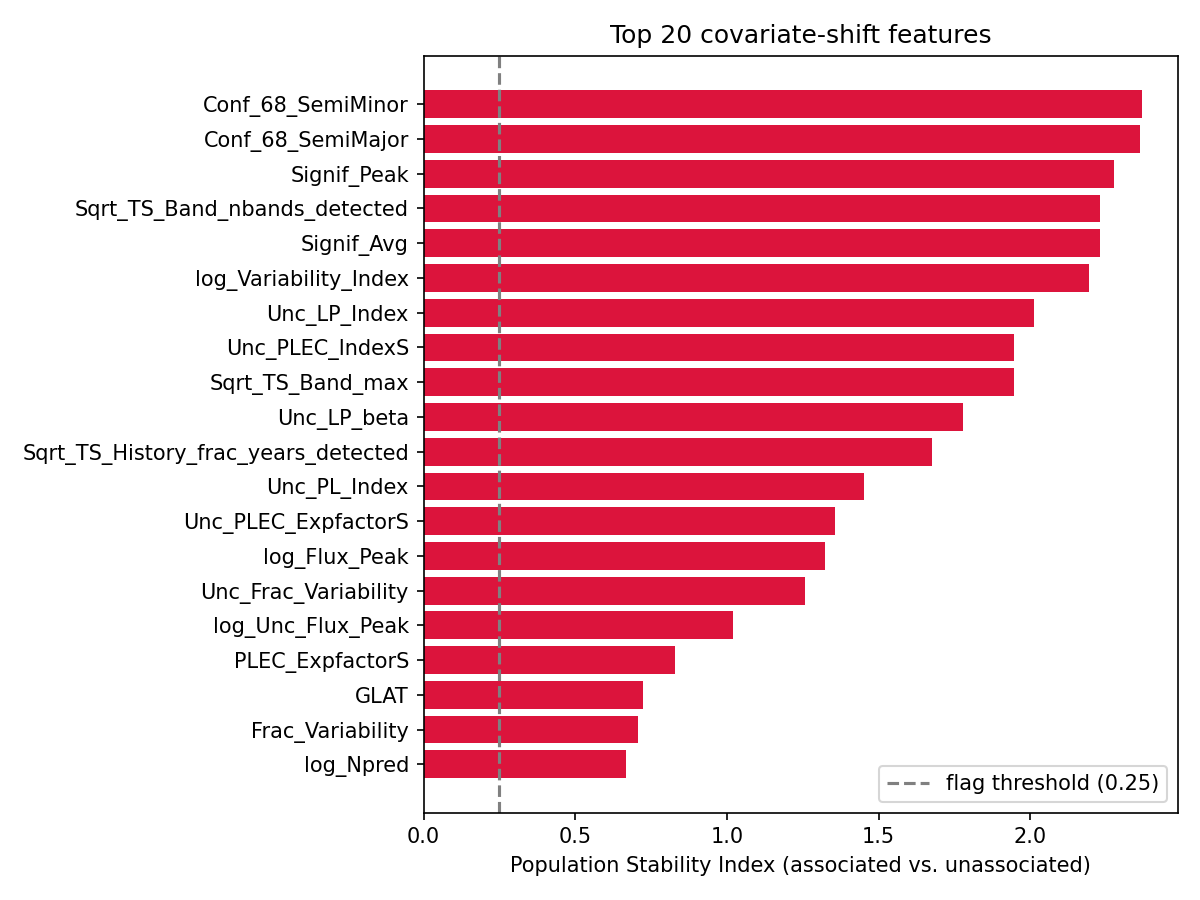
\includegraphics[width=\linewidth]{covariate_shift.png}
    \end{column}
    \begin{column}{0.48\textwidth}
      \small
      \begin{itemize}
        \item KS test and population stability index (PSI) per feature, associated against
              unassociated.
        \item 33 of 65 features are flagged: both the KS test and PSI \(>\) 0.25.
        \item The largest shifts are in significance, localization and detection: unassociated
              sources are fainter and more often in the Galactic plane.
        \item Test-set scores therefore overstate performance on the unassociated sources.
              This is measured in the results.
      \end{itemize}
    \end{column}
  \end{columns}
\end{frame}

\begin{frame}{Model search}
  \begin{itemize}\small
    \item Models: logistic regression, random forest, HistGBC, CatBoost, three MLPs; LDA on the
          two smallest branches. Default hyperparameters.
    \item For each model: choose the feature set, then the class weighting (none, balanced,
          dampened, balanced without cap).
    \item Coarse-to-fine: a quick screen on a 15\% holdout, then 5-fold stratified CV for the
          survivors.
    \item Hierarchies are scored end to end with chain CV: router, gate and branches are refit
          inside every fold, so routing errors are counted.
    \item Selection metric: macro-F1. Balanced accuracy ignores false positives; an earlier run
          selected on it and sent hundreds of \cls{bll} and \cls{fsrq} into rare classes.
  \end{itemize}
\end{frame}

\begin{frame}{Validation and choice of the winners}
  \begin{enumerate}\small
    \item Shortlist the best candidates per family (5 flat, 15 merged, 27 three-level
          combinations).
    \item Re-score the shortlist on the training data and keep the top 5 per family.
    \item Pick one winner per family with a Borda count: average rank over accuracy, balanced
          accuracy, macro-F1 and \(\kappa\), plus the gap between training and CV scores as an
          overfitting penalty.
    \item Score the three winners once on the test set, with 95\% bootstrap intervals,
          per-class metrics, calibration and shift checks.
  \end{enumerate}
  \vspace{0.2cm}
  \small Disclosure: the reduced search space was chosen from the CV leaderboards of an earlier
  run on a different split, so some of those rows are in today's test set. The choice was coarse
  (which model families to keep), so the effect should be small.
\end{frame}

% =====================================================================
\section{Results}

\begin{frame}{Main result}
  \centering\scriptsize
  \begin{tabular}{llccc}
    \toprule
    Family & Deployed model & CV macro-F1 & Test macro-F1 [95\% CI] & Test accuracy \\
    \midrule
    Flat & Logistic regression, 10 features & 0.291 & 0.319 [0.287, 0.354] & 0.832 \\
    2-level & RF router; RF, LR, LDA, CatBoost branches & 0.284 & 0.329 [0.268, 0.373] & 0.819 \\
    3-level & MLP gate and sub-gate; CatBoost router & 0.295 & 0.309 [0.270, 0.346] & 0.829 \\
    \bottomrule
  \end{tabular}

  \vspace{0.25cm}
  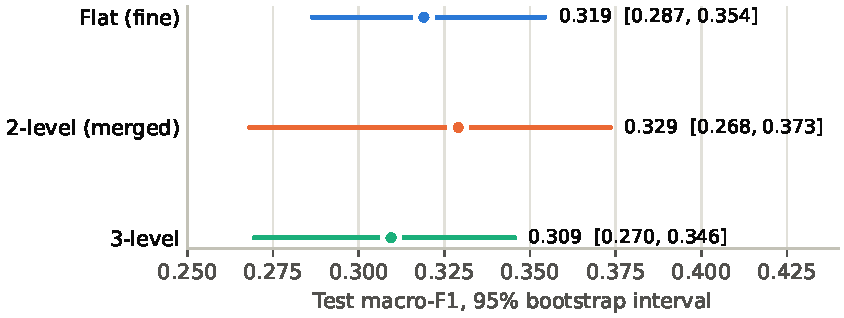
\includegraphics[width=0.55\linewidth]{family_macro_f1.pdf}
  \begin{itemize}\small
    \item The intervals overlap almost entirely. No architecture is better than the others, and
          the hierarchies do not beat a flat logistic regression.
  \end{itemize}
\end{frame}

\begin{frame}{Training, CV and test scores}
  \centering
  \begin{tabular}{lccc}
    \toprule
    Macro-F1 & Training & CV & Test \\
    \midrule
    Flat & 0.335 & 0.291 & 0.319 \\
    2-level & 0.920 & 0.284 & 0.329 \\
    3-level & 0.585 & 0.295 & 0.309 \\
    \bottomrule
  \end{tabular}
  \vspace{0.4cm}
  \begin{itemize}\small
    \item The 2-level model fits the training data almost perfectly (random-forest router) and
          generalizes no better than the flat model.
    \item CV and test agree within the intervals for all three families, so the selection was
          not optimistic.
    \item The flat model is simpler and much less overfit, which makes it the sensible choice
          when the scores are tied.
  \end{itemize}
\end{frame}

\begin{frame}{Where the errors are}
  \begin{columns}[c]
    \begin{column}{0.52\textwidth}
      \centering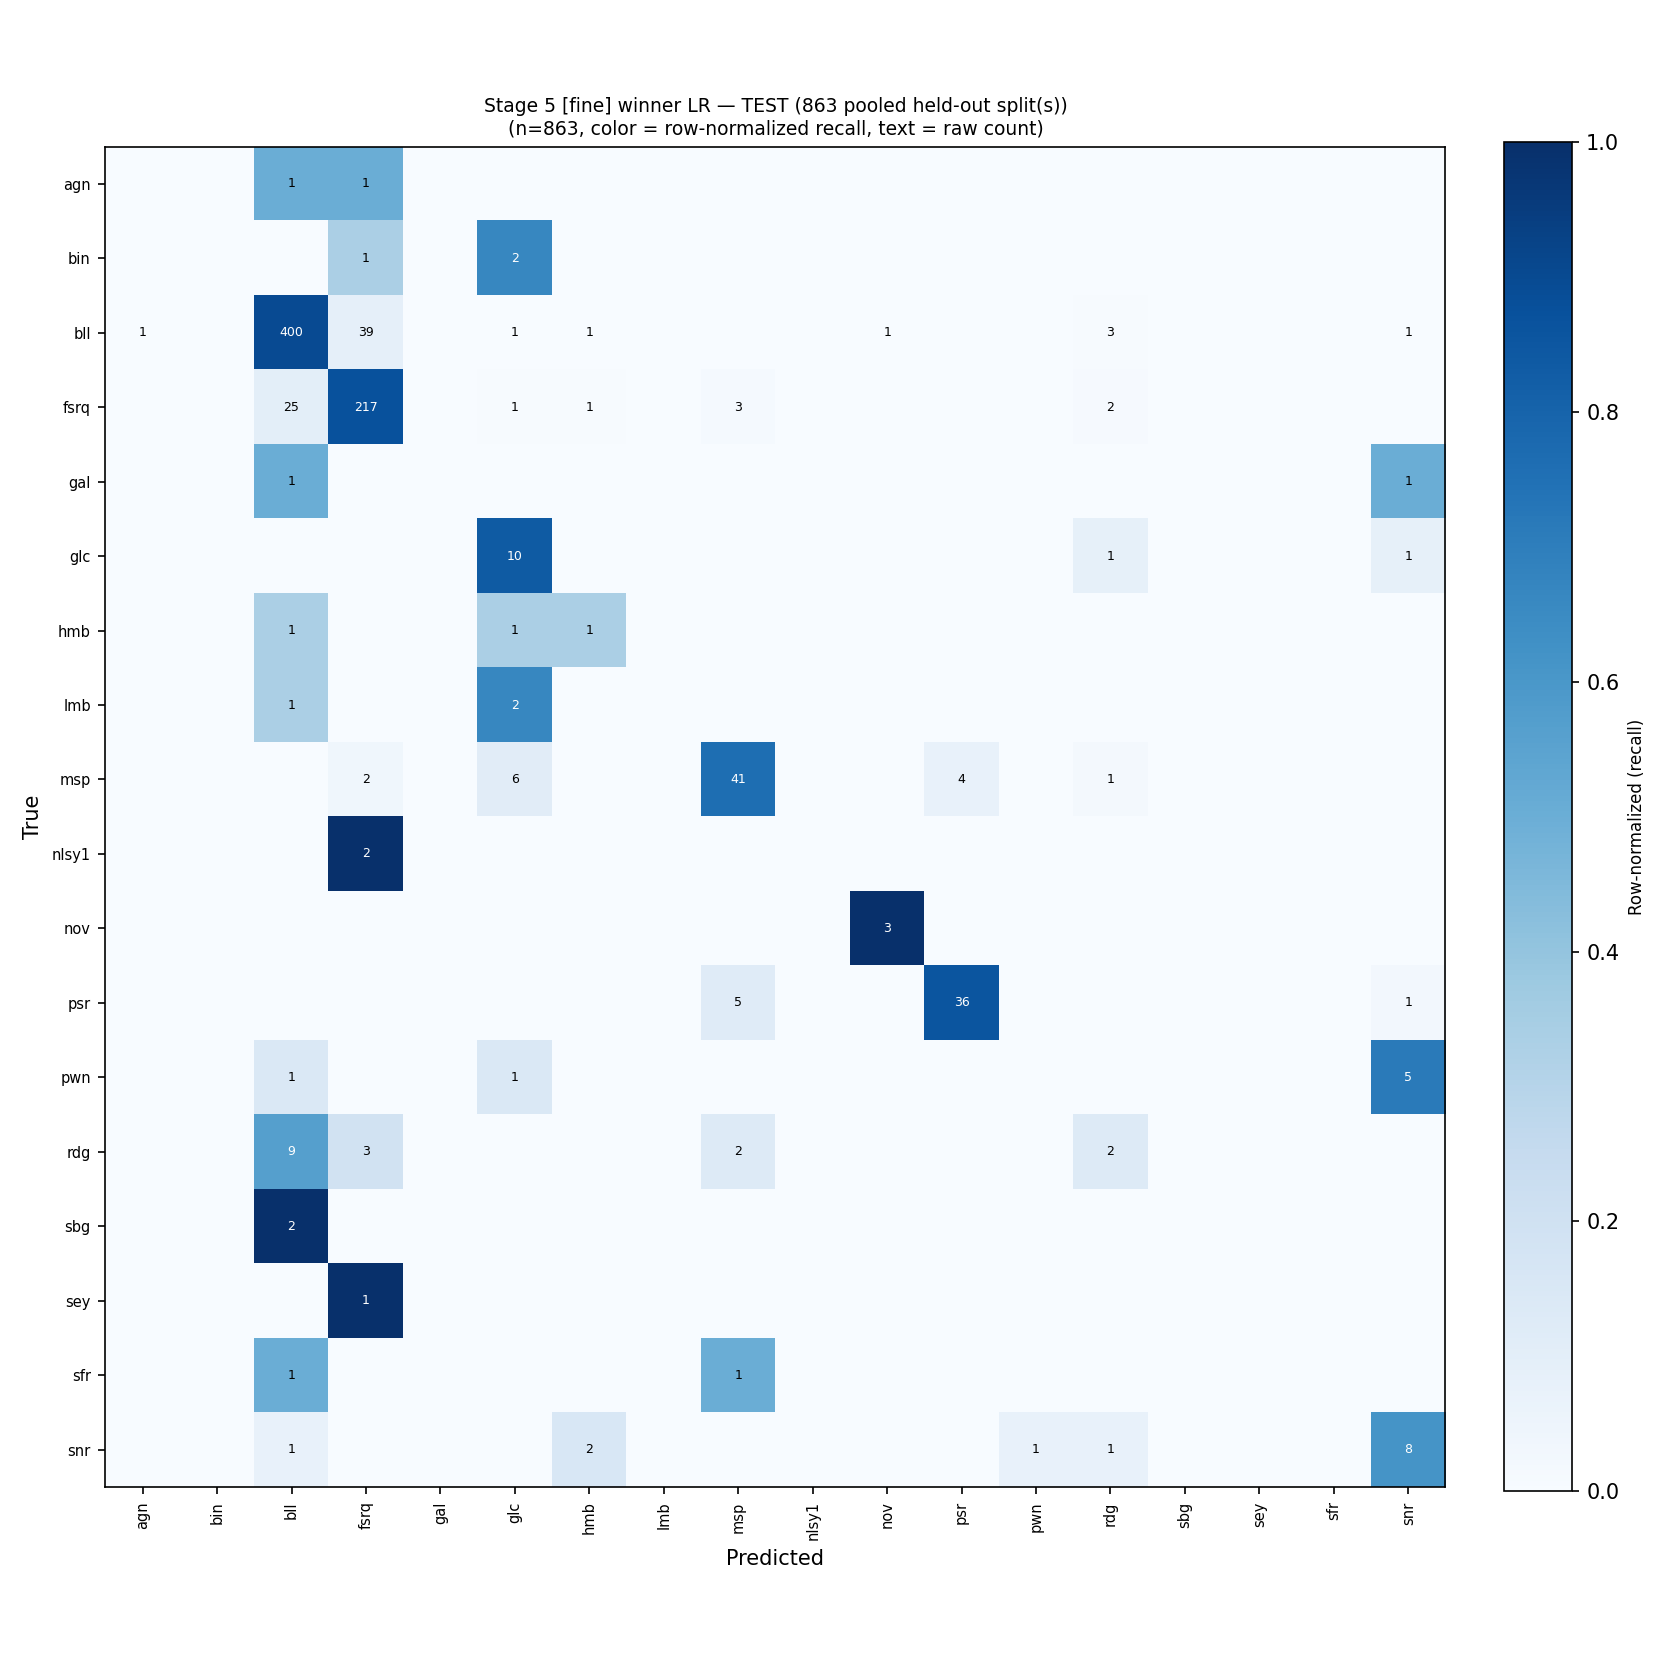
\includegraphics[height=0.84\textheight]{confusion_fine_test.png}
    \end{column}
    \begin{column}{0.46\textwidth}
      \small
      Flat model on the 863 test sources (colour: recall per true class).
      \begin{itemize}
        \item The main error is between the two blazar classes: 39 \cls{bll} predicted as
              \cls{fsrq}, 25 \cls{fsrq} as \cls{bll}.
        \item Pulsars are separated well (\cls{psr} 36 of 42, \cls{msp} 41 of 54).
        \item Radio galaxies (\cls{rdg}) mostly go to \cls{bll}.
        \item Most rare classes are absorbed by the large ones.
      \end{itemize}
    \end{column}
  \end{columns}
\end{frame}

\begin{frame}{Results per class (test F1)}
  \begin{columns}[T]
    \begin{column}{0.5\textwidth}
      \centering\scriptsize
      \begin{tabular}{lrccc}
        \toprule
        Class & n & Flat & 2-level & 3-level \\
        \midrule
        \cls{bll} & 447 & 0.90 & 0.89 & 0.89 \\
        \cls{fsrq} & 249 & 0.84 & 0.81 & 0.82 \\
        \cls{msp} & 54 & 0.77 & 0.71 & 0.76 \\
        \cls{psr} & 42 & 0.88 & 0.80 & 0.89 \\
        \cls{rdg} & 16 & 0.15 & 0.00 & 0.00 \\
        \cls{snr} & 13 & 0.53 & 0.77 & 0.71 \\
        \cls{glc} & 12 & 0.56 & 0.38 & 0.38 \\
        \cls{pwn} & 7 & 0.00 & 0.67 & 0.62 \\
        \cls{hmb} & 3 & 0.25 & 0.40 & 0.50 \\
        \cls{nov} & 3 & 0.86 & 0.00 & 0.00 \\
        \cls{lmb} & 3 & 0.00 & 0.50 & 0.00 \\
        \cls{bin} & 3 & 0.00 & 0.00 & 0.00 \\
        6 other classes & 1 or 2 & 0.00 & 0.00 & 0.00 \\
        \bottomrule
      \end{tabular}
    \end{column}
    \begin{column}{0.47\textwidth}
      \small
      \begin{itemize}
        \item The four large classes reach F1 0.71 to 0.90 in every family.
        \item The hierarchies help supernova remnants and pulsar wind nebulae, and lose globular
              clusters and novae.
        \item With 1 to 3 test sources, one source moves F1 by a large step: the lower half of
              the table cannot rank the families.
      \end{itemize}
    \end{column}
  \end{columns}
\end{frame}

\begin{frame}{Are the probabilities trustworthy?}
  \begin{columns}[c]
    \begin{column}{0.42\textwidth}
      \centering
      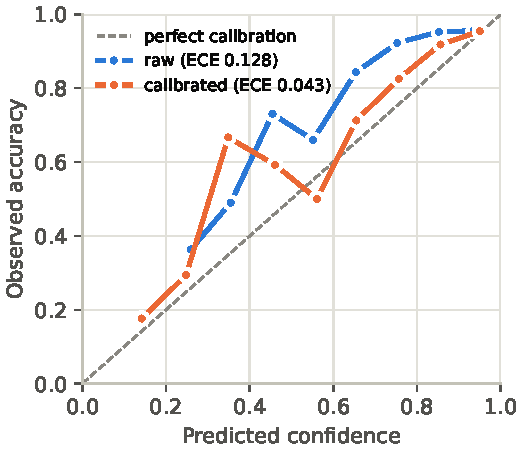
\includegraphics[width=0.95\linewidth]{reliability_fine.pdf}
    \end{column}
    \begin{column}{0.56\textwidth}
      \small
      \begin{tabular}{lcc}
        \toprule
        Model & Brier & ECE \\
        \midrule
        Flat, raw & 0.285 & 0.128 \\
        Flat, calibrated & 0.254 & 0.043 \\
        2-level, raw & 0.276 & 0.060 \\
        3-level, raw & 0.247 & 0.023 \\
        \bottomrule
      \end{tabular}
      \begin{itemize}
        \item The raw flat model is underconfident: class weighting moves probability toward
              rare classes.
        \item Undoing the weighting and one temperature, fit on out-of-fold training
              predictions, fixes most of it.
        \item The 3-level model is close to calibrated as it is.
      \end{itemize}
    \end{column}
  \end{columns}
\end{frame}

\begin{frame}{How well does it transfer to unassociated sources?}
  \centering\small
  \begin{tabular}{lrcc}
    \toprule
    Flat model, test subset & n & Accuracy & Macro-F1 \\
    \midrule
    All test sources & 863 & 0.832 & 0.319 \\
    \(|b| < 10^\circ\) (Galactic plane) & 127 & 0.732 & 0.439 \\
    \(|b| \ge 10^\circ\) & 736 & 0.849 & 0.241 \\
    Signif\_Avg \(< 4.9\) (faint) & 39 & 0.590 & 0.307 \\
    Signif\_Avg \(\ge 6.8\) (bright) & 709 & 0.859 & 0.317 \\
    Reweighted to look like the unassociated sources & \(\approx\)50 eff. & 0.430 & 0.180 \\
    \bottomrule
  \end{tabular}
  \vspace{0.3cm}
  \begin{itemize}\small
    \item Faint and Galactic-plane sources are harder, and the unassociated population is full of
          them.
    \item Importance-weighted to that population, accuracy drops from 0.83 to about 0.43 (all
          three families: 0.43 to 0.46). The estimate is rough (effective sample about 50), but the
          direction is clear.
  \end{itemize}
\end{frame}

\begin{frame}{Check against a later catalog release}
  \begin{columns}[c]
    \begin{column}{0.5\textwidth}
      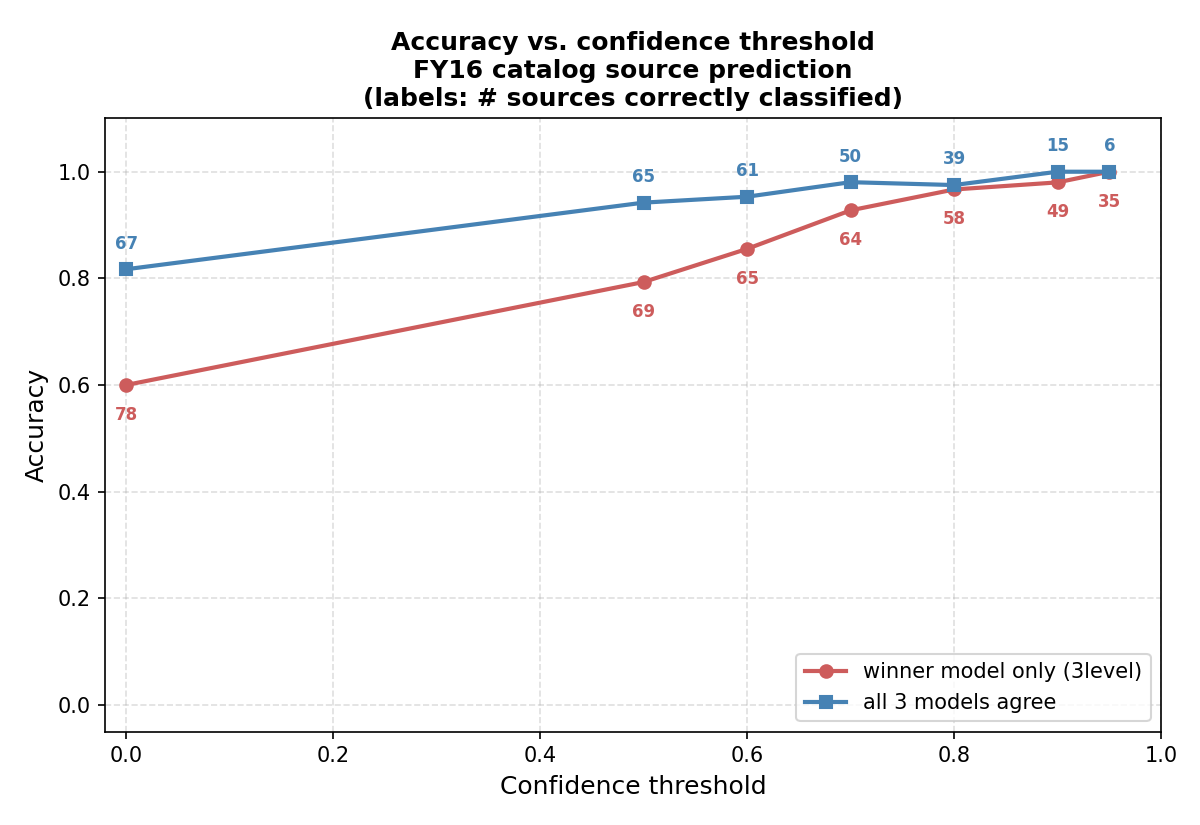
\includegraphics[width=\linewidth]{v41_accuracy_vs_confidence.png}
    \end{column}
    \begin{column}{0.48\textwidth}
      \scriptsize
      \begin{tabular}{lrc}
        \toprule
        Subset & n & Accuracy [95\% CI] \\
        \midrule
        3-level, all & 130 & 0.60 [0.51, 0.69] \\
        3-level, confidence \(\ge\) 0.8 & 60 & 0.97 [0.89, 1.00] \\
        All 3 agree & 82 & 0.82 [0.72, 0.89] \\
        All 3 agree, each \(\ge\) 0.7 & 51 & 0.98 [0.90, 1.00] \\
        \bottomrule
      \end{tabular}
      \small
      \begin{itemize}
        \item \cls{gll\_psc\_v41} has since associated some DR4 unassociated sources: a test the
              models never saw (\cls{bcu}, \cls{spp}, \cls{unk} excluded).
        \item Confidence and agreement between families both sort good predictions from bad.
        \item The newly associated sources need not represent the rest.
      \end{itemize}
    \end{column}
  \end{columns}
\end{frame}

% =====================================================================
\section{Conclusions}

\begin{frame}{Conclusions}
  \begin{enumerate}\small
    \item On held-out data the three architectures are tied: test macro-F1 0.31 to 0.33 with
          overlapping intervals. A flat logistic regression on 10 features is as good as the
          hierarchies and overfits far less.
    \item The large classes are learned well (F1 0.77 to 0.90 for \cls{bll}, \cls{fsrq},
          \cls{msp}, \cls{psr}); most rare classes are not, and their scores rest on 1 to 3
          test sources.
    \item Performance on the unassociated sources is much lower than the test score suggests,
          because they are fainter and more Galactic.
    \item Confident predictions on which all three families agree are reliable on the later
          catalog: 0.98 accuracy on 51 sources.
  \end{enumerate}
\end{frame}

\begin{frame}{Limitations and next steps}
  \begin{columns}[T]
    \begin{column}{0.5\textwidth}
      \small Limitations
      \begin{itemize}\small
        \item One split: intervals cover test-row sampling, not split-to-split variation.
        \item Default hyperparameters.
        \item The search space was narrowed using an earlier run on a different split.
        \item Calibration and prior correction exist for the flat model only.
      \end{itemize}
    \end{column}
    \begin{column}{0.5\textwidth}
      \small Next steps
      \begin{itemize}\small
        \item Repeat search and selection on 5 splits (already implemented).
        \item Correct the class priors for the unassociated population; add a reject option.
        \item Ablation without sky position (\cls{GLAT}, \cls{GLON}).
        \item Per-class report of the later-catalog check.
      \end{itemize}
    \end{column}
  \end{columns}
  \vspace{0.3cm}
  \small Full list: \cls{TODO.md} in the repository.
\end{frame}

\begin{frame}{Code and documentation}
  \begin{itemize}
    \item Repository: \url{https://github.com/filippo-graci/fermi-4fgl-classification}
    \item \cls{README.md}: what the pipeline does and how to run it.
    \item \cls{RESULTS.md}: all results with methodology and caveats.
    \item \cls{docs/scientific\_review\_with\_citations.md}: every step with its justification and
          literature.
    \item \cls{outputs\_.../validation/csv\_reports/}: every number in this talk.
  \end{itemize}
  \vspace{0.6cm}
  \centering\Large Thank you
\end{frame}

\end{document}
